\begin{itemframe}{‌مسئلهٔ پوشش رأسی}
\itm
مسئله پوشش رأسی
\fn{vertex cover problem}
یک مسئلهٔ ان‌پی کامل است.
\itm
پوشش رأسی یک گراف بدون جهت
$G = (V,E)$
زیر مجموعه‌ای از رئوس گراف
$V' \subseteq V$
است به طوری‌که اگر
$(u,v)$
یک یال از گراف
$G$
باشد، آنگاه
$u \in V'$
یا
$v \in V'$
یا هردو. اندازه پوشش رأسی تعداد رأس‌های
$V'$
است.
\itm
در مسئلهٔ پوشش رأسی می‌خواهیم کمترین تعداد رئوس در یک گراف را پیدا کنیم که یک پوشش رأسی تشکیل می‌دهند یا به عبارت دیگر همهٔ یال‌ها را پوشش می دهند. به چنین پوشش رأسی یک پوشش رأسی بهینه
\fn{optimal vertex cover}
می‌گوییم.
\itm
اگرچه هیچ الگوریتم چند جمله‌ای برای مسئلهٔ پوشش رأسی یافته نشده است، اما یک الگوریتم تقریبی چندجمله‌ای برای پیدا کردن جواب نزدیک به بهینه وجود دارد.
\end{itemframe}


\begin{itemframe}{‌مسئلهٔ پوشش رأسی}
\itm
الگوریتم تقریبی زیر یک گراف بدون جهت را دریافت می‌کند و یک پوشش رأسی باز می‌گرداند که اندازهٔ آن کمتر از دو برابر پوشش رأسی بهینه است.
\begin{algorithm}[H]\alglr
  \caption{Approx-Vertex-Cover}
  \begin{algorithmic}[1]
   \Func{Approx-Vertex-Cover}{G}
   \State C = $\emptyset$
   \State E' = G.E
   \While{E' $\neq \emptyset$}
   			\State let (u,v) be an arbitrary edge of E'
   			\State C = C $\cup$ \{(u,v)\}
   			\State remove from E' edge (u,v) and every edge incident on either u or v
   	\EndWhile
   	\State \Return C
  \end{algorithmic}
  \label{alg:merge}
\end{algorithm}
\itm
متغیر
$C$
پوشش رأسی در حال ساخت را نگه می‌دارد. این الگوریتم با لیست مجاورت در زمان
$O(|V|+|E|)$
اجرا می‌شود.
\end{itemframe}


\begin{itemframe}{‌مسئلهٔ پوشش رأسی}
\itm
شکل زیر نشان می‌دهد این الگوریتم چگونه برروی یک گراف عمل می‌کند.
در پایان این الگوریتم تقریبی ۶ رأس را برای پوشش رأسی پیدا می‌کند در صورتی که جواب بهینه برای این نمونه مسئله ۳ است.
\begin{figure}
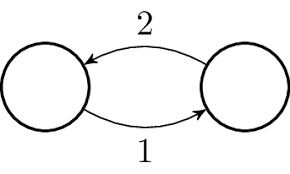
\includegraphics[width=0.3\textwidth]{figs/\chapdir/1}
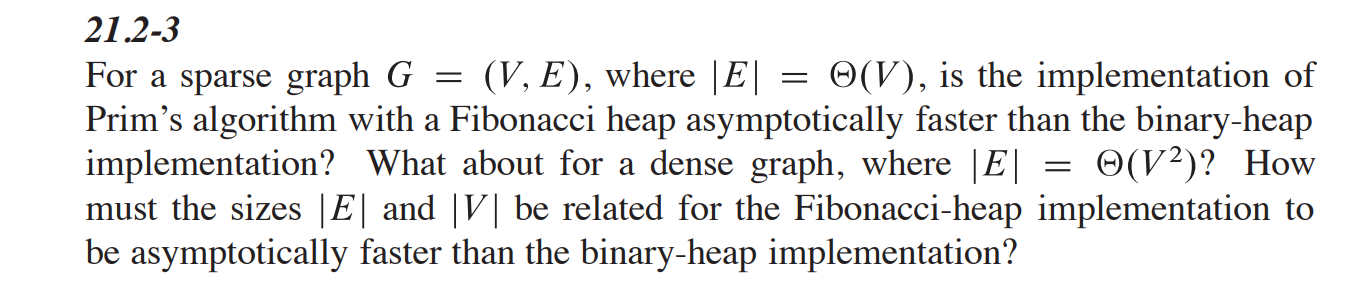
\includegraphics[width=0.6\textwidth]{figs/\chapdir/2}
\end{figure}
\end{itemframe}


\begin{itemframe}{‌مسئلهٔ پوشش رأسی}
\item[\textbullet]
قضیه : الگوریتم تقریبی پوشش رأسی یک الگوریتم چند جمله‌ای تقریبی با ضریت ۲ است.
\item[\textbullet]
اثبات : مجموعهٔ
$C$
یک پوشش رأسی است زیرا الگوریتم در حلقه تا وقتی تکرار می‌شود که همهٔ یال‌های
$G.E$
با یکی از رئوس
$C$
پوشش داده شده‌اند.
\item[\textbullet]
حال می‌خواهیم ثابت کنیم این الگوریتم یک الگوریتم تقریبی با ضریب ۲ است.
\item[\textbullet]
فرض کنید
$A$
مجموعه‌ای از یال‌ها باشد که در خط ۴ الگوریتم انتخاب شده‌اند. برای اینکه یال‌های مجموعه
$A$
پوشش داده شوند، هر پوشش رأسی باید حداقل یکی از دو رأس هریال در
$A$
را شامل شود. هیچ دو یالی در
$A$
رأس مشترک ندارند، زیرا وقتی یک یال در خط ۴ انتخاب شد، همهٔ یال‌هایی که با آن یال رأس مشترک دارند از مجموعه
$E'$
در خط ۶ حذف می‌شوند.
\end{itemframe}
\iffalse

\begin{itemframe}{‌مسئلهٔ پوشش رأسی}
\itm
بنابراین هیچ دویالی در
$A$
با یک رأس از
$C^*$
پوشش داده نشده‌اند و این بدین معنی است که به ازای هر رأس در
$C^*$
، حداکثر یک یال در
$A$
وجود دارد و بنابراین داریم :
\begin{align*}
$|C^*| \geqslant |A|$
\end{align*}
\itm
هر اجرای خط ۴ یک یال را انتخاب \می‌کند که هیچ‌کدام از دو رأس مجاور آن در
$C$
نیستند و بنابراین داریم :
\begin{align*}
$|C| = 2 |A|$
\end{align*}
\itm
با استفاده از دو رابطهٔ به دست آمده خواهیم داشت :
\begin{align*}
$|C| = 2 |A| \leqslant 2|C^*|$
\end{align*}
و قضیه بدین ترتیب اثبات می‌شود.
\end{itemframe}
\fi